 
\chapter{Generalized Estimating Equation for Correlated Multivariate Data}\label{chapter::gee}
 
Previous chapters dealt with cross-sectional data, that is, we observe $n$ units at a particular time point, collecting various covariates and outcomes. In addition, we assume that these units are independent, and sometimes, we even assume they are IID draws. Many applications have correlated data. Two canonical examples are 
\begin{enumerate}
[(E1)]
\item
repeated measurements of the same set of units over  time, which are often called {\it longitudinal data} in biostatistics \citep{fitzmaurice2012applied} or {\it panel data} in econometrics \citep{wooldridge2010econometric}; and
\item
clustered observations belonging to classrooms, villages, etc, which are common in cluster-randomized experiments in education \citep{schochet2013estimators} and public health \citep{turner2017reviewdesign, turner2017reviewanalysis}. 
\end{enumerate}
Many excellent textbooks cover this topic intensively. This chapter focuses on a simple yet powerful strategy, which is a natural extension of the GLM discussed in the last chapter. It was initially proposed in \citet{liang1986longitudinal}, the most cited paper published in {\it Biometrika} in the past one hundred years \citep{titterington2013biometrika}. 
For simplicity, we will use the term ``longitudinal data'' for general correlated data. 


 
 
\section{Examples of correlated data} 
 
 
 
\subsection{Longitudinal data}

We have used the data from \citet{royer2015incentives} in Chapter \ref{chapter::count}. Each worker's number of gym visits was repeatedly measured over more than 100 weeks. It is a standard longitudinal dataset. In Chapter \ref{chapter::count}, we conducted analysis for each week separately, and in this chapter, we will accommodate the longitudinal structure of the data. 



\subsection{Clustered data: a neuroscience experiment} 


\citet{moen2016analyzing} examined the effects of Pten knockdown and fatty acid delivery on soma size of neurons in the brain of a mouse. The useful variables for our analysis are the id of mouse \ri{mouseid}, the fatty acid level \ri{fa}, the Pten knockdown indicator \ri{pten}, the outcome \ri{somasize}, the number of neurons \ri{numpten} and \ri{numctrl} under Pten knockdown or not.


\begin{lstlisting}
> Pten = read.csv("PtenAnalysisData.csv")[, -(7:9)]
> head(Pten)
  mouseid fa pten somasize numctrl numpten
1       0  0    0   83.837      30      44
2       0  0    0   69.984      30      44
3       0  0    0   82.128      30      44
4       0  0    0   86.446      30      44
5       0  0    0   74.032      30      44
6       0  0    0   71.693      30      44
\end{lstlisting}

The three-way table below shows the treatment combinations for 14 mice, from which
we can see that the Pten knockdown indicator varies within mice, but the fatty acid level varies only between mice. 
\begin{lstlisting}
> table(Pten$mouseid, Pten$fa, Pten$pten)
, ,  = 0

    
      0  1  2
  0  30  0  0
  1  58  0  0
  2  18  0  0
  3   2  0  0
  4  56  0  0
  5   0 39  0
  6   0 33  0
  7   0 58  0
  8   0 60  0
  9   0  0 15
  10  0  0 27
  11  0  0  7
  12  0  0 34
  13  0  0 22

, ,  = 1

    
      0  1  2
  0  44  0  0
  1  68  0  0
  2  33  0  0
  3  11  0  0
  4  76  0  0
  5   0 55  0
  6   0 55  0
  7   0 75  0
  8   0 92  0
  9   0  0 34
  10  0  0 29
  11  0  0 20
  12  0  0 53
  13  0  0 38
  \end{lstlisting}


\subsection{Clustered data: a public health intervention} 



Poor sanitation leads to morbidity and mortality in developing countries. In 2012, \citet{guiteras2015encouraging} conducted a cluster-randomized experiment in rural Bangladesh to evaluate the effectiveness of different policies on the use of hygienic latrines. To illustrate our theory, we use a subset of their original data and exclude the households not eligible for subsidies or with missing outcomes, resulting in 10125 households in total. The median, mean, and maximum of village size are 83, 119, and 500, respectively.
We choose the outcome $y_{it}$ as the binary indicator for whether the household $(i,t)$ had access to a hygienic latrine or not, measured in June 2013, and covariate $x_{it}$ as the baseline access rate to hygienic latrines in the community that household $(i,t)$ belonged to, measured in January 2012 before the experiment.

The useful variables below are \ri{z}, \ri{x}, \ri{y}, and \ri{vid}, which denote the binary treatment indicator, covariate $x_{it}$, the outcome, and the village id \ri{vid}, 
\begin{lstlisting}
> hygaccess = read.csv("hygaccess.csv")
> hygaccess = hygaccess[,c("r4_hyg_access", "treat_cat_1", 
+                          "bl_c_hyg_access", "vid", "eligible")]
> hygaccess = hygaccess[which(hygaccess$eligible=="Eligible"&
+                               hygaccess$r4_hyg_access!="Missing"),]
> hygaccess$y = ifelse(hygaccess$r4_hyg_access=="Yes", 1, 0)
> hygaccess$z = hygaccess$treat_cat_1
> hygaccess$x = hygaccess$bl_c_hyg_access
\end{lstlisting}



\section{Marginal model and the generalized estimating equation}

We will extend the restricted mean model to deal with longitudinal
data, where we observe outcome $y_{it}$ and covariate $x_{it}$ for
each unit $i=1,\ldots,n$ at time $t=1,\ldots,n_{i}.$ The $n_i$'s can vary across units. When $n_{i}=1$
for all units, we drop the time index and model the conditional mean
as 
\[
E(y_{i}\mid x_{i})=\mu(x_{i}^{\T}\beta),
\]
and use the following estimating equation  
to estimate the parameter $\beta$:
\begin{equation}
\sumn\frac{y_{i}-\mu(x_{i}^{\T}\beta)}{\tilde{\sigma}^{2}(x_{i}, \beta)}\frac{\partial\mu(x_{i}^{\T}\beta)}{\partial\beta}=0 . \label{eq:quasi-likelihood-gee-chapter}
\end{equation}
In \eqref{eq:quasi-likelihood-gee-chapter},  $\tilde{\sigma}^{2}(x_{i}, \beta)$ is a working variance function usually motivated by a GLM, but it can be misspecified. With an $n_{i}\times1$ vector outcome and  an $n_{i}\times p$ covariate matrix
\begin{eqnarray}
\label{eq::individual-y-x}
Y_{i} = \begin{pmatrix}
y_{i1} \\
\vdots \\
y_{in_{i}}
\end{pmatrix},\quad 
X_{i} = \begin{pmatrix}
x_{i1}^{\T} \\
\vdots \\
x_{in_{i}}^{\T}
\end{pmatrix},\quad
(i=1,\ldots, n)
\end{eqnarray}
we can extend the restricted mean model to
\begin{eqnarray}
E(Y_{i}\mid X_{i}) 
&\equiv& \left(\begin{array}{c}
E(y_{i1}\mid X_{i})\\
\vdots\\
E(y_{in_{i}}\mid X_{i})
\end{array}\right)  \label{eq::def1-gee} \\
&=& \left(\begin{array}{c}
E(y_{i1}\mid x_{i1})\\
\vdots\\
E(y_{in_{i}}\mid x_{in_{i}})
\end{array}\right)  \label{eq::gee-assumtion-1} \\
&=&\left(\begin{array}{c}
\mu(x_{i1}^{\T}\beta)\\
\vdots\\
\mu(x_{in_{i}}^{\T}\beta)
\end{array}\right)   \label{eq::gee-assumtion-2} \\
&\equiv&\mu(X_{i},\beta), \label{eq::def2-gee}
\end{eqnarray}
where \eqref{eq::def1-gee} and \eqref{eq::def2-gee} are definitions, and \eqref{eq::gee-assumtion-1} and \eqref{eq::gee-assumtion-2}
are the two key assumptions. Assumption \eqref{eq::gee-assumtion-1} requires that the conditional mean of $y_{it}$ depends only on $x_{it}$
but not on any other $x_{is}$ with $s\neq t$. Assumption \eqref{eq::gee-assumtion-2} requires
that the relationship between $x_{it}$ and $y_{it}$ is stable across units and time points with the function $\mu(\cdot)$ and the parameter
$\beta$ not varying with respect to $i$ or $t$. The model assumptions in \eqref{eq::gee-assumtion-1} and \eqref{eq::gee-assumtion-2} 
are really strong, and I defer the critiques to the end of this chapter.
Nevertheless, the marginal model attracts practitioners for 
\begin{enumerate}
[({A}1)]
\item\label{advantage-1}
its similarity to GLM and the restricted mean model, and
\item \label{advantage-2}
its simplicity of requiring only specification of the marginal conditional
means, not the whole joint distribution. 
\end{enumerate}
The advantage (A\ref{advantage-1}) facilitates
the interpretation of the coefficient, and the advantage (A\ref{advantage-2}) is crucial
because of the lack of familiar multivariate distributions in statistics
except for the multivariate Normal. The generalized estimating equation
(GEE) for $\beta$ is the vector form of (\ref{eq:quasi-likelihood-gee-chapter}):
\begin{equation}
\sumn\underbrace{\frac{\partial\mu (X_{i},\beta)}{\partial\beta}}_{p\times n_{i}}
\underbrace{\tilde{V}^{-1}(X_{i},\beta)}_{n_{i}\times n_{i}}
\underbrace{\left\{ Y_{i}-\mu(X_{i},\beta)\right\} }_{n_{i}\times1}
= \underbrace{0}_{p\times 1},\label{eq:gee-liang-zeger-form}
\end{equation}
where (\ref{eq:gee-liang-zeger-form}) has a similar form as (\ref{eq:quasi-likelihood-gee-chapter})
with three terms organized to match the dimension so that matrix multiplications
are well-defined:
\begin{enumerate}
[(GEE1)]
\item the last term 
\[
Y_{i}-\mu(X_{i},\beta)=\left(\begin{array}{c}
y_{i1} -\mu(x_{i1}^{\T}\beta)\\
\vdots\\
y_{in_{i}} -\mu(x_{in_{i}}^{\T}\beta)
\end{array}\right)
\]
represents the residual vector,
\item the second term is the inverse of $\tilde{V}(X_{i}, \beta)$, a working covariance
matrix of the conditional distribution of $Y_{i}$ given $X_{i}$
which may be misspecified:
\[
\tilde{V}(X_{i}, \beta)\neq V(X_{i})\equiv\cov(Y_{i}\mid X_{i}).
\]
It is relatively easy to specify the working variance $\tilde{\sigma}^2(x_{it}, \beta)$ for each marginal component, for example, based on the marginal GLM.  So the key is to specify the $n_i\times n_i$ dimensional correlation matrix $R_i$ to obtain 
$$
\tilde{V}(X_{i}, \beta) = \text{diag}\{ \tilde{\sigma} (x_{it}, \beta) \}_{i=1}^{n_i} R_i \text{diag}\{ \tilde{\sigma} (x_{it}, \beta) \}_{i=1}^{n_i}.
$$
We assume that the $R_i$'s are given now, and will discuss how to choose them in a later section. 
\item the first term is the partial derivative of an $n_i \times 1$ 
vector $\mu (X_{i},\beta)=(\mu(x_{i1}^{\T}\beta),\ldots,\mu(x_{in_{i}}^{\T}\beta))^{\T}$
with respect to a $p\times1$ vector $\beta=(\beta_{1},\ldots,\beta_{p})^{\T}$:
\begin{eqnarray*}
\frac{\partial\mu (X_{i},\beta)}{\partial\beta}
&=& \left(  \frac{\partial \mu(x_{i1}^{\T}\beta)}{\partial \beta},\ldots,  \frac{ \partial  \mu(x_{in_{i}}^{\T}\beta)}{\partial \beta} \right)  \\
&=&\left(\begin{array}{ccc}
\frac{\partial\mu(x_{i1}^{\T}\beta)}{\partial\beta_{1}} & \cdots & \frac{\partial\mu(x_{in_{i}}^{\T}\beta)}{\partial\beta_{1}}\\
\vdots &  & \vdots\\
\frac{\partial\mu(x_{i1}^{\T}\beta)}{\partial\beta_{p}} & \cdots & \frac{\partial\mu(x_{in_{i}}^{\T}\beta)}{\partial\beta_{p}}
\end{array}\right),
\end{eqnarray*}
which is a $p\times n_i$ matrix, denoted by $D_{i} (\beta).$
\end{enumerate}

\section{Statistical inference with GEE}

\subsection{Computation using the Gauss--Newton method\label{subsec:Computation-gee-gauss-newton}}

We can use Newton's method to solve the GEE (\ref{eq:gee-liang-zeger-form}).
However, calculating the derivative of the left-hand side of (\ref{eq:gee-liang-zeger-form})
involves calculating the second order derivative of $ \mu (X_{i},\beta)$ with respect to $\beta$.
A simpler alternative without calculating the second-order derivative
is the Gauss--Newton method based on the following approximation:
\begin{align*}
0 & =\sumn\frac{\partial\mu (X_{i},\beta)}{\partial\beta}\tilde{V}^{-1}(X_{i})\left\{ Y_{i}-\mu(X_{i},\beta)\right\} \\
 & \cong \sumn D_{i} (\beta^{\text{old}})\tilde{V}^{-1}(X_{i}, \beta^{\text{old}})\left[\left\{ Y_{i}-\mu(X_{i},\beta^{\text{old}})\right\} -D_{i}^{\T}(\beta^{\text{old}})(\beta-\beta^{\text{old}})\right]\\
 & =\sumn D_{i} (\beta^{\text{old}})\tilde{V}^{-1}(X_{i}, \beta^{\text{old}})\left\{ Y_{i}-\mu(X_{i},\beta^{\text{old}})\right\} \\
 & \quad -\sumn D_{i} (\beta^{\text{old}})\tilde{V}^{-1}(X_{i}, \beta^{\text{old}})D_{i}^{\T}(\beta^{\text{old}})(\beta-\beta^{\text{old}}) . 
\end{align*}
So given $\beta^{\text{old}}$, we update it as
\begin{eqnarray}
\beta^{\text{new}} &=& \beta^{\text{old}}
+\left\{ \sumn D_{i} (\beta^{\text{old}})\tilde{V}^{-1}(X_{i}, \beta^{\text{old}})D_{i}^{\T}(\beta^{\text{old}})\right\} ^{-1} \nonumber \\
&& \times 
\sumn D_{i} (\beta^{\text{old}})\tilde{V}^{-1}(X_{i}, \beta^{\text{old}})\left\{ Y_{i}-\mu(X_{i},\beta^{\text{old}})\right\} . 
\label{eq::gauss-newton-gee}
\end{eqnarray}


\subsection{Asymptotic inference\label{subsec:Asymptotic-inference-GEE}}

The asymptotic distribution of $\hat{\beta}$ follows from Theorem \ref{theorem:sandwich-theorem-cov-ind}. Similar to the proof of Theorem \ref{theorem::glm-sandwich}, we can verify that $\sqrt{n}(\hat{\beta}-\beta)\rightarrow\N(0,B^{-1}MB^{-1})$
in distribution where
\begin{align*}
B & =E\left\{ n^{-1}\sumn  D_{i} (\beta)\tilde{V}^{-1}(X_{i}, \beta)D_{i}^{\T}(\beta)\right\} ,\\
M & =E\left\{ n^{-1}\sumn D_{i} (\beta)\tilde{V}^{-1}(X_{i}, \beta)V(X_{i})\tilde{V}^{-1}(X_{i}, \beta)D_{i}^{\T}(\beta)\right\} .
\end{align*}
After obtaining $\hat{\beta}$ and the residual vector $\hat{\varepsilon}_{i}=Y_{i}-\mu(X_{i},\hat{\beta})$
for unit $i$ $(i=1,\ldots,n)$, we can conduct asymptotic inference
based on the Normal approximation 
\[
\hat{\beta}\asim\N(\beta,n^{-1}\hat{B}^{-1}\hat{M}\hat{B}^{-1}),
\]
where 
\begin{align*}
\hat{B} & =n^{-1}\sumn D_{i} (\hat{\beta})\tilde{V}^{-1}(X_{i}, \hat{\beta})D_{i}^{\T}(\hat{\beta}),\\
\hat{M} & =n^{-1}\sumn D_{i} (\hat{\beta})\tilde{V}^{-1}(X_{i}, \hat{\beta})\hat{\varepsilon}_{i}\hat{\varepsilon}_{i}^{\T}\tilde{V}^{-1}(X_{i}, \hat{\beta})D_{i}^{\T}(\hat{\beta}).
\end{align*}
This covariance estimator proposed by \citet{liang1986longitudinal}, is robust to the misspecification of the marginal variances and the correlation structure as long as the conditional mean of $Y_i$ given $X_i$ is correctly specified.  




\subsection{Implementation: choice of the working covariance matrix}

We have not discussed the choice of the working correlation matrix
$R_i$. Different choices do not affect the consistency
but affect the efficiency of $\hat{\beta}$. A simple starting point
is the independent working correlation matrix $R_i = I_{n_i}$.
Under this correlation matrix, the GEE reduces to
\begin{eqnarray*}
\sumn \left(  \frac{ \partial  \mu(x_{i1}^{\T}\beta)}{\partial \beta},\ldots,  \frac{ \partial   \mu(x_{in_{i}}^{\T}\beta)}{\partial \beta} \right) 
\left(\begin{array}{ccc}
\tilde{\sigma}^{-2}(x_{i1}, \beta)\\
 & \ddots\\
 &  & \tilde{\sigma}^{-2}(x_{in_{i}}, \beta)
\end{array}\right) \\
\times 
\left(\begin{array}{c}
 y_{i1} -\mu(x_{i1}^{\T}\beta)\\
\vdots\\
 y_{in_{i}} -\mu(x_{in_{i}}^{\T}\beta)
\end{array}\right) =0,
\end{eqnarray*}
or, more compactly,
\begin{eqnarray}
\label{eq::independent-working-cov-gee}
\sumn\sum_{t=1}^{n_{i}}\frac{y_{it}-\mu(x_{it}^{\T}\beta)}{\tilde{\sigma}^{2}(x_{it}, \beta)}\frac{\partial\mu(x_{it}^{\T}\beta)}{\partial\beta}=0.
\end{eqnarray}
This is simply the estimating equation of a restricted mean model
treating all data points $(i,t)$ as independent observations. This
implies that the point estimate assuming the independent working correlation matrix is still consistent, although we must change the standard error
as in Section \ref{subsec:Asymptotic-inference-GEE}. 

With this simple starting point, we have a consistent yet inefficient
estimate of $\beta$, and then we can compute the residuals. The correlation
among the residuals contains information about the true covariance
matrix. With small and equal $n_{i}$'s, we can estimate the conditional
covariance without imposing any structure based on the residuals.
Using the estimated covariance matrix, we can update the GEE estimate
to improve efficiency. This leads to a two-step procedure. 

An important intermediate case is motivated by the exchangeability
of the data points within the same unit $i$, so the working covariance
matrix is $\tilde{V}(X_{i}, \beta)= \text{diag}\{\tilde{\sigma}(x_{it})\}_{i=1}^{n_i} R_i(\rho) \text{diag}\{\tilde{\sigma}(x_{it})\}_{i=1}^{n_i} $, where
\[
R_i(\rho) = \left(\begin{array}{cccc}
1 & \rho & \cdots & \rho\\
\rho & 1 & \cdots & \rho\\
\vdots & \vdots &  & \vdots\\
\rho & \rho & \cdots & 1
\end{array}\right) .
\]
We can estimate $\rho$ based on the residuals from the first step.

The above three choices of the working covariance matrix are called
``\ri{independent}'', ``\ri{unstructured}'', and ``\ri{exchangeable}'' in the ``\ri{corstr}''
parameter of the function \ri{gee} in the \ri{gee} package in \ri{R}. This function
also contains other choices proposed by \citet{liang1986longitudinal}. 


A carefully chosen working covariance matrix can lead to efficiency gain compared to the simple independent covariance matrix. An efficient estimator requires a correctly specified working covariance matrix. This is often an infeasible goal, and what is more, the conditional covariance $\cov(Y_i\mid X_i)$ is a nuisance parameter if the conditional mean is the main parameter of interest. In practice, the independent working covariance suffices in many applications despite its potential efficiency loss. This is similar to the use of OLS in the presence of heteroskedasticity in linear models. Section \ref{sec::crse-econometrics} focuses on the independent working covariance, which is common in econometrics. Section \ref{sec::critiquesonGEEassumptions} gives further justifications for this simple strategy. 



\section{A special case: cluster-robust standard error} 
\label{sec::crse-econometrics}


Importantly, \citet{liang1986longitudinal}'s standard error treats each cluster $i$ as an independent contributor to the uncertainty. In econometrics, this is called the cluster-robust standard error. Alternatively, we can use the bootstrap by resampling the clusters to approximate the asymptotic covariance matrix.
I will discuss linear and logistic regressions in this section, and leave the technical details of Poisson regression as a homework problem. 




Stack the $Y_i$'s and $X_i$'s in \eqref{eq::individual-y-x} together to obtain 
$$
Y = \begin{pmatrix}
Y_1 \\
\vdots \\
Y_n
\end{pmatrix},\quad
X = \begin{pmatrix}
X_1 \\
\vdots \\
X_n
\end{pmatrix},
$$
which are the $N$ dimensional outcome vector and $N\times p$ covariate matrix, where $N = \sumn n_i.$


\subsection{OLS}\label{sec::crse-ols}

An important special case is the
marginal linear model with an independent working covariance matrix
and homoskedasticity, resulting in the following estimating equation:
\[
\sumn\sum_{t=1}^{n_{i}}x_{it}(y_{it}-x_{it}^{\T}\beta)=0.
\]
So the point estimator is just the pooled OLS using all data
points:
\begin{align*}
\hat{\beta} & =\left(\sumn\sum_{t=1}^{n_{i}}x_{it}x_{it}^{\T}\right)^{-1}\sumn\sum_{t=1}^{n_{i}}x_{it}y_{it}\\
 & =\left(\sumn X_{i}^{\T}X_{i}\right)^{-1}\sumn X_{i}^{\T}Y_{i} \\
 &= (X^{\T} X)^{-1} X^{\T} Y.
\end{align*}
The three forms of $\hat{\beta} $ above are identical: the first one is based on $N$ observations, the second one is based on $n$ independent units, and the last one is based on the matrix form with the pooled data. 
Although the point estimate is identical to the case with independent
data points, we must adjust for the standard error according to Section
\ref{subsec:Asymptotic-inference-GEE}. From
$$
D_i(\beta) = ( x_{i1}, \ldots, x_{in_i} ) = X_i^{\T},
$$
we can verify that
\[
\hat{\cov}(\hat{\beta})=\left(\sumn X_{i}^{\T}X_{i}\right)^{-1}\sumn X_{i}^{\T}\hat{\varepsilon}_{i}\hat{\varepsilon}_{i}^{\T}X_{i}\left(\sumn X_{i}^{\T}X_{i}\right)^{-1},
\]
where $\hat{\varepsilon}_{i}=Y_{i}-X_{i}\hat{\beta}=(\hat{\varepsilon}_{i1},\ldots,\hat{\varepsilon}_{in_{i}})^{\T}$
is the residual vector of unit $i$. This is called the (Liang--Zeger) cluster-robust
covariance matrix in econometrics. The square roots of the diagonal terms are called the cluster-robust standard errors. 
The cluster-robust
covariance matrix is often much larger than the
(Eicker--Huber--White) heteroskedasticity-robust covariance matrix assuming
independence of observations $(i,t)$:
\[
\hat{\cov}_{\textsc{ehw}}(\hat{\beta})=\left(\sumn\sum_{t=1}^{n_{i}}x_{it}x_{it}^{\T}\right)^{-1}\sumn\sum_{t=1}^{n_{i}}\hat{\varepsilon}_{it}^{2}x_{it}x_{it}^{\T}\left(\sumn\sum_{t=1}^{n_{i}}x_{it}x_{it}^{\T}\right)^{-1}.
\]
Note that 
$$
X^{\T} X = \sumn X_{i}^{\T}X_{i} = \sumn\sum_{t=1}^{n_{i}}x_{it}x_{it}^{\T},
$$ 
so the bread matrices in $\hat{\cov}(\hat{\beta})$ and $\hat{\cov}_{\textsc{ehw}}(\hat{\beta})$ are identical. The only difference is due to the meat matrices:
$$
\sumn X_{i}^{\T}\hat{\varepsilon}_{i}\hat{\varepsilon}_{i}^{\T}X_{i}
= \sumn  \left( \sum_{t=1}^{n_{i}}\hat{\varepsilon}_{it} x_{it}\right) \left( \sum_{t=1}^{n_{i}}\hat{\varepsilon}_{it} x_{it} \right)^{\T}
\neq \sumn\sum_{t=1}^{n_{i}}\hat{\varepsilon}_{it}^{2}x_{it}x_{it}^{\T}
$$
in general. 


\subsection{Logistic regression}\label{sec::crse-logit}

For binary outcomes, we can use the marginal logistic model with an independent working covariance matrix,
resulting in the following estimating equation:
\[
\sumn\sum_{t=1}^{n_{i}}x_{it} \left\{ y_{it}-  \pi(x_{it}, \beta)\right\} =0
\]
where $ \pi(x_{it}, \beta) =  e^{x_{it}^{\T}\beta} / (1+e^{x_{it}^{\T}\beta} )  .$
So the point estimator is  the pooled logistic regression using all data
points, but we must adjust for the standard error according to Section
\ref{subsec:Asymptotic-inference-GEE}. From
\begin{eqnarray*}
D_i(\beta) &=&  (
 \pi(x_{i1}, \beta) \{1- \pi(x_{i1}, \beta)\} x_{i1}, \ldots, 
 \pi(x_{in_i}, \beta)\{1- \pi(x_{in_i}, \beta)\} x_{in_i} 
) \\
&=&  X_i^{\T} \tilde{V}(X_i, \beta),
\end{eqnarray*}
with $ \tilde{V}(X_i, \beta) = \text{diag}\{  \pi(x_{it}, \beta) \{1- \pi(x_{it}, \beta)\} \}_{t=1}^{n_i}$,
we can verify that
$$
\hat{B} = n^{-1} \sumn X_i^{\T}  \hat{V}_i X_i,\quad
\hat{M} = n^{-1} \sumn X_i^{\T}  \hat{\varepsilon}_i   \hat{\varepsilon}_i^{\T} X_i,
$$
where $\hat{\varepsilon}_{i} = (\hat{\varepsilon}_{i1}, \ldots, \hat{\varepsilon}_{in_i})^{\T}$ with residual
$\hat{\varepsilon}_{it}=y_{it}-e^{x_{it}\hat{\beta}}/(1+e^{x_{it}\hat{\beta}}) $, and $\hat{V}_i = \text{diag}\{  \pi(x_{it}, \hat{\beta}) \{1- \pi(x_{it}, \hat{\beta})\} \}_{t=1}^{n_i}.$
So the cluster-robust covariance estimator for logistic regression is
\[
\hat{\cov}(\hat{\beta})=\left(\sumn X_{i}^{\T} \hat{V}_i X_{i}\right)^{-1}
\sumn X_{i}^{\T}\hat{\varepsilon}_{i}\hat{\varepsilon}_{i}^{\T}X_{i}
\left(\sumn X_{i}^{\T} \hat{V}_i X_{i}\right)^{-1}.
\]
 

I leave the cluster-robust covariance estimator for Poisson regression to Problem \ref{hw21::poisson-crse}. 



\section{Application}

We will use the \ri{gee} package for all the analyses below. 
%The \ri{R} code is in 

 



\subsection{Clustered data: a neuroscience experiment} 


The original study was interested in the potential interaction between two treatments, so I always include the interaction term in the regression model. 


From the simple specification below, \ri{pten} has a significant effect, but \ri{fa} and the interactions are not significant.
\begin{lstlisting}
 Pten.gee = gee(somasize ~ factor(fa)*pten, 
+                id = mouseid, 
+                family = gaussian, 
+                corstr = "independence",
+                data = Pten)
> summary(Pten.gee)$coef 
                 Estimate Naive S.E. Naive z Robust S.E. Robust z
(Intercept)        93.106      1.594 58.4216       3.059  30.4374
factor(fa)1         3.756      2.175  1.7268       3.174   1.1836
factor(fa)2         6.907      2.551  2.7078       5.407   1.2774
pten               11.039      2.082  5.3016       2.200   5.0166
factor(fa)1:pten    8.727      2.834  3.0795       5.023   1.7373
factor(fa)2:pten   -2.904      3.270 -0.8881       3.554  -0.8173
> 
> 
> Pten.gee = gee(somasize ~ factor(fa)*pten, 
+                id = mouseid, 
+                family = gaussian, 
+                corstr = "exchangeable",
+                data = Pten)
> summary(Pten.gee)$coef
                 Estimate Naive S.E. Naive z Robust S.E. Robust z
(Intercept)        90.900      3.532 25.7376       2.701  33.6535
factor(fa)1         4.921      5.115  0.9621       2.914   1.6889
factor(fa)2         6.408      5.066  1.2649       5.904   1.0853
pten               11.501      1.979  5.8120       2.190   5.2515
factor(fa)1:pten    8.807      2.688  3.2766       5.050   1.7439
factor(fa)2:pten   -1.525      3.113 -0.4898       2.703  -0.5641
\end{lstlisting}
 
 
 
Including two covariates, we have the following results. The covariates are predictive of the outcome, changing the significance level of the main effect of \ri{fa}.  The interaction terms between \ri{pten} and \ri{fa} are not significant either. 
\begin{lstlisting}
> Pten.gee = gee(somasize ~ factor(fa)*pten + numctrl + numpten, 
+                id = mouseid, 
+                family = gaussian, 
+                corstr = "independence",
+                data = Pten)
> summary(Pten.gee)$coef 
                 Estimate Naive S.E. Naive z Robust S.E. Robust z
(Intercept)       81.9422      2.791 29.3602      4.0917   20.026
factor(fa)1        6.2267      2.237  2.7835      4.2429    1.468
factor(fa)2       14.8956      2.657  5.6053      4.1839    3.560
pten              12.3771      2.020  6.1272      2.2477    5.507
numctrl            0.8721      0.120  7.2672      0.3028    2.880
numpten           -0.4843      0.101 -4.7948      0.2381   -2.034
factor(fa)1:pten   7.7498      2.744  2.8240      5.1064    1.518
factor(fa)2:pten  -2.9629      3.166 -0.9359      3.3105   -0.895
>  
> 
> Pten.gee = gee(somasize ~ factor(fa)*pten + numctrl + numpten, 
+                id = mouseid, 
+                family = gaussian, 
+                corstr = "exchangeable",
+                data = Pten)
> summary(Pten.gee)$coef
                 Estimate Naive S.E. Naive z Robust S.E. Robust z
(Intercept)       85.3316     5.2872 16.1393      5.4095  15.7745
factor(fa)1        5.4952     4.2761  1.2851      4.0207   1.3667
factor(fa)2       12.2174     4.1669  2.9320      4.2363   2.8840
pten              11.8044     1.9718  5.9865      2.1946   5.3789
numctrl            0.9326     0.2867  3.2527      0.3479   2.6810
numpten           -0.5678     0.2504 -2.2674      0.2772  -2.0482
factor(fa)1:pten   8.5137     2.6777  3.1795      5.0612   1.6821
factor(fa)2:pten  -1.7755     3.0995 -0.5728      2.7547  -0.6445
\end{lstlisting}
 
 
From the regressions above, we observe that (1) two choices of the covariance matrix do not lead to fundamental differences; and (2) without using the cluster-robust standard error, the results can be misleading. 
 
 
 \subsection{Clustered data: a public health intervention} 

We first fit simple GEE without using the covariate.
\begin{lstlisting}
> hygaccess.gee = gee(y ~ z, id = vid,
+                     family = binomial(link = logit),
+                     corstr = "independence", 
+                     data = hygaccess)
> summary(hygaccess.gee)$coef
                    Estimate Naive S.E. Naive z Robust S.E. Robust z
(Intercept)          -0.7568    0.04439 -17.049      0.1763  -4.2924
zLPP Only             0.1551    0.06657   2.330      0.2301   0.6741
zLPP+Subsidy          0.7562    0.05503  13.742      0.2027   3.7313
zLPP+Subsidy+Supply   0.7344    0.05444  13.490      0.2010   3.6546
zSupply Only          0.3568    0.07364   4.846      0.3091   1.1544
> 
> hygaccess.gee = gee(y ~ z, id = vid,
+                     family = binomial(link = logit),
+                     corstr = "exchangeable", 
+                     data = hygaccess)
> summary(hygaccess.gee)$coef
                    Estimate Naive S.E. Naive z Robust S.E. Robust z
(Intercept)          -0.7799     0.1314 -5.9371      0.1522  -5.1235
zLPP Only             0.1638     0.2042  0.8021      0.2290   0.7152
zLPP+Subsidy          0.7789     0.1500  5.1926      0.1790   4.3524
zLPP+Subsidy+Supply   0.7348     0.1506  4.8798      0.1760   4.1753
zSupply Only          0.2690     0.2207  1.2187      0.3011   0.8931
\end{lstlisting}


Without adjusting for the covariates, treatment levels ``zLPP+Subsidy'' and ``zLPP+Subsidy+Supply'' are significant. The \ri{exchangeable} working covariance matrix does seem to improve the estimated precision. 


We then fit GEE with a covariate. 

\begin{lstlisting}
> hygaccess.gee = gee(y ~ z + x, id = vid,
+                     family = binomial(link = logit),
+                     corstr = "independence", 
+                     data = hygaccess)
> summary(hygaccess.gee)$coef
                    Estimate Naive S.E. Naive z Robust S.E. Robust z
(Intercept)          -1.7526    0.06174 -28.386      0.1398  -12.538
zLPP Only             0.2277    0.06833   3.332      0.1393    1.635
zLPP+Subsidy          0.6850    0.05645  12.133      0.1191    5.749
zLPP+Subsidy+Supply   0.7389    0.05578  13.246      0.1361    5.430
zSupply Only          0.3614    0.07514   4.810      0.2426    1.490
x                     2.0488    0.08209  24.957      0.2158    9.492
> 
> hygaccess.gee = gee(y ~ z + x, id = vid,
+                     family = binomial(link = logit),
+                     corstr = "exchangeable", 
+                     data = hygaccess)
> summary(hygaccess.gee)$coef
                    Estimate Naive S.E. Naive z Robust S.E. Robust z
(Intercept)          -1.7976     0.1324 -13.575      0.1541  -11.667
zLPP Only             0.3038     0.1781   1.705      0.1946    1.561
zLPP+Subsidy          0.7227     0.1316   5.491      0.1271    5.688
zLPP+Subsidy+Supply   0.8547     0.1327   6.441      0.1247    6.855
zSupply Only          0.3236     0.1911   1.693      0.2398    1.350
x                     1.9497     0.1128  17.286      0.1947   10.016
\end{lstlisting}

Covariate adjustment improves efficiency and makes the choice of the working covariance matrix less important. 

 
 
 
\subsection{Longitudinal data}


The regression formula \ri{f.reg} will remain the same although other parameters may vary. 

\begin{lstlisting}
> library("gee")
> library("foreign")
> gym1 = read.dta("gym_treatment_exp_weekly.dta")
> f.reg = weekly_visit ~ incentive_commit + incentive + target + member_gym_pre
\end{lstlisting}


Using all data, we find a significant effect of \ri{incentive_commit} but an insignificant effect of \ri{incentive}. 

\begin{lstlisting}
 normal.gee = gee(f.reg, id = id, 
+                family = gaussian, 
+                corstr = "independence", 
+                data = gym1)
> normal.gee = summary(normal.gee)$coef
> normal.gee
                 Estimate Naive S.E. Naive z Robust S.E. Robust z
(Intercept)      -0.69005   0.011136 -61.968     0.08672  -7.9572
incentive_commit  0.15666   0.008358  18.745     0.06376   2.4569
incentive         0.01022   0.008275   1.235     0.05910   0.1729
target            0.62666   0.007465  83.949     0.06773   9.2527
member_gym_pre    1.14919   0.007077 162.375     0.06252  18.3801
\end{lstlisting}

However, this pooled analysis can be misleading because we have seen from the analysis before that the treatments have no effects in the pre-experimental periods and smaller effects in the long term. A pooled analysis can dilute the short-term effects, missing the treatment effect heterogeneity across time. This can be fixed by the following subgroup analysis based on time.

\begin{lstlisting}
> normal.gee1 = gee(f.reg, id = id, 
+                  subset = (incentive_week<0),
+                  family = gaussian, 
+                  corstr = "independence", 
+                  data = gym1)
> normal.gee1 = summary(normal.gee1)$coef
> normal.gee1
                  Estimate Naive S.E.  Naive z Robust S.E.  Robust z
(Intercept)      -0.879374    0.04230 -20.7868     0.08739 -10.06224
incentive_commit -0.004241    0.03175  -0.1336     0.06243  -0.06794
incentive        -0.073884    0.03144  -2.3502     0.06223  -1.18728
target            0.742675    0.02836  26.1887     0.06701  11.08301
member_gym_pre    1.601569    0.02689  59.5664     0.06600  24.26763
>  
> 
> normal.gee2 = gee(f.reg, id = id, 
+                   subset = (incentive_week>0&incentive_week<15),
+                   family = gaussian, 
+                   corstr = "independence", 
+                   data = gym1)
> normal.gee2 = summary(normal.gee2)$coef  
> normal.gee2
                 Estimate Naive S.E. Naive z Robust S.E. Robust z
(Intercept)       -0.7925    0.03275 -24.194     0.08982   -8.823
incentive_commit   0.3662    0.02458  14.898     0.06895    5.311
incentive          0.1744    0.02434   7.166     0.06457    2.701
target             0.6735    0.02196  30.674     0.07159    9.408
member_gym_pre     1.4138    0.02082  67.914     0.06727   21.018
> 
> normal.gee3 = gee(f.reg, id = id, 
+                   subset = (incentive_week>=15),
+                   family = gaussian, 
+                   corstr = "independence", 
+                   data = gym1)
> normal.gee3 = summary(normal.gee3)$coef
> normal.gee3
                  Estimate Naive S.E. Naive z Robust S.E. Robust z
(Intercept)      -0.661500   0.012222  -54.13     0.09028  -7.3273
incentive_commit  0.134789   0.009173   14.69     0.06676   2.0189
incentive        -0.009716   0.009082   -1.07     0.06142  -0.1582
target            0.611635   0.008193   74.66     0.07042   8.6860
member_gym_pre    1.077874   0.007768  138.77     0.06494  16.5967
\end{lstlisting} 

Changing the \ri{family} parameter to \ri{poisson(link = log)}, we can fit a marginal log-linear model with independent Poisson covariance. Figure \ref{fig::gee-analysis-gym-data} shows the point estimates and confidence intervals based on the regressions above. The confidence intervals based on the cluster-robust standard errors are much wider than those based on the EHW standard errors. Without dealing with clustering, the confidence intervals are too narrow and give wrong inference.

\begin{figure}[ht]
\centering
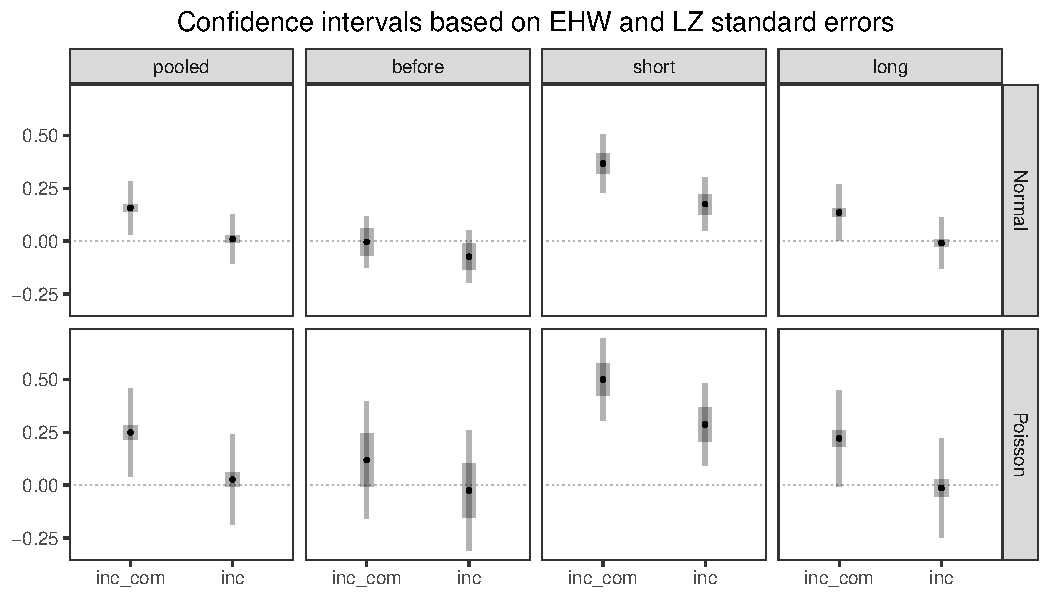
\includegraphics[width=\textwidth]{figures/ci_ehw_lz_gym.pdf}
\caption{GEE analysis of the gym data}\label{fig::gee-analysis-gym-data}
\end{figure}



\section{Critiques on the key assumptions}
\label{sec::critiquesonGEEassumptions}
Consider the simple case with $n_i=2$ for all $i$ below. 

\subsection{Assumption \eqref{eq::gee-assumtion-1}} 

Assumption \eqref{eq::gee-assumtion-1} requires
$$
E(y_{it} \mid X_i) = E(y_{it} \mid x_{it}) , 
$$
which holds automatically if $x_{it} = x_i$ is time-invariant. With time-varying covariates, it effectively rules out the dynamics between $x$ and $y$. Assumption \eqref{eq::gee-assumtion-1} holds in the following data-generating process:
$$
\xymatrix{
x_{i1} \ar[r]\ar[d] &x_{i2} \ar[d] \\
y_{i1} & y_{i2}
}
$$
It does not hold if the lagged $x$ affects $y$ or the lagged $y$ affects $x$:
$$
\xymatrix{
x_{i1} \ar[r]\ar[d]\ar[dr] &x_{i2} \ar[d] \\
y_{i1} & y_{i2}
}
\qquad 
\text{ or }
\qquad 
\xymatrix{
x_{i1} \ar[r]\ar[d] &x_{i2} \ar[d] \\
y_{i1} \ar[ur] & y_{i2}
}
\qquad 
\text{ or }
\qquad 
\xymatrix{
x_{i1} \ar[r]\ar[d]\ar[dr] &x_{i2} \ar[d] \\
y_{i1} \ar[ur] & y_{i2}
}
$$
With more complex data generating processes, Assumption \eqref{eq::gee-assumtion-1} does not hold in general:
$$
\xymatrix{
x_{i1} \ar[r]\ar[d]\ar[dr] &x_{i2} \ar[d] \\
y_{i1} \ar[ur] \ar[r] & y_{i2}
}
$$

\citet{liang1986longitudinal} assumed fixed covariates, ruling out the dynamics of $x$.
\citet{sullivan1994cautionary} pointed out the importance of Assumption \eqref{eq::gee-assumtion-1} in GEE with random time-varying covariates. \citet{sullivan1994cautionary}  also showed that with an independent working covariance matrix, we can drop Assumption \eqref{eq::gee-assumtion-1} as long as the marginal conditional mean is correctly specified. That is, if $E(y_{it}\mid x_{it}) = \mu(x_{it}^{\T}\beta)$, then 
\begin{eqnarray*}
&&E\left\{ \sumn\sum_{t=1}^{n_{i}}\frac{y_{it}-\mu(x_{it}^{\T}\beta)}{\tilde{\sigma}^{2}(x_{it}, \beta)}\frac{\partial\mu(x_{it}^{\T}\beta)}{\partial\beta} \right\}  \\
% &=& 
% \sumn\sum_{t=1}^{n_{i}}  E\left\{  \frac{y_{it}-\mu(x_{it}^{\T}\beta)}{\tilde{\sigma}^{2}(x_{it}, \beta)}\frac{\partial\mu(x_{it}^{\T}\beta)}{\partial\beta} \right\} \\ 
 &=&\sumn\sum_{t=1}^{n_{i}}  E\left[ \frac{ E\{ y_{it}-\mu(x_{it}^{\T}\beta) \mid x_{it} \} }{\tilde{\sigma}^{2}(x_{it}, \beta)}\frac{\partial\mu(x_{it}^{\T}\beta)}{\partial\beta} \right] \\
 &=& 0.
\end{eqnarray*}
This gives another justification for the use of the independent working covariance matrix even though it can result in efficiency loss when Assumption \eqref{eq::gee-assumtion-1} holds. 


\subsection{Assumption \eqref{eq::gee-assumtion-2}} 


Assumption \eqref{eq::gee-assumtion-2} requires a ``stable'' relationship between $x$ and $y$ across clusters and time points:
$$
E(y_{it} \mid x_{it}) = \mu(x_{it}^{\T} \beta)
$$ 
where $\mu$ and $\beta$ do not depend on $i$ or $t$. 
For clustered data, we can justify this assumption by the exchangeability of the units within clusters. However, it is much harder to interpret or justify it for longitudinal data with complex outcome dynamics. 

We consider linear structural equations with a scalar time-invariant covariate. Without direct dependence of $y_{i2}$ on $y_{i1}$, the data generating process
\begin{eqnarray*}
y_{i1} &=& \alpha_1 + \beta  x_i  + \varepsilon_{i1},\\
y_{i2} &=& \alpha_2 + \beta x_i  + \varepsilon_{i2},
\end{eqnarray*}
corresponding to the graph
$$
\xymatrix{
&x_{i} \ar[dl]  \ar[dr] &  \\
y_{i1}   && y_{i2} 
}
$$
has conditional expectations $E(y_{it}\mid x_{i}) =  \alpha_t +  \beta  x_i   $ if 
\begin{equation}
\label{eq::exogenous-gee}
  E(\varepsilon_{it}\mid x_i) = 0.
\end{equation}
However, with direct dependence of $y_{i2}$ on $y_{i1}$, the data generating process
\begin{eqnarray*}
y_{i1} &=& \alpha_1 +  \beta x_i  + \varepsilon_{i1},\\
y_{i2} &=& \alpha_2 +  \gamma  y_{i1}   + \delta x_i   + \varepsilon_{i2},
\end{eqnarray*}
corresponding to the graph
$$
\xymatrix{
&x_{i} \ar[dl]  \ar[dr] &  \\
y_{i1}  \ar[rr] && y_{i2} 
}
$$
has conditional expectations $E(y_{i1}\mid x_{i}) = \alpha_1 +  \beta   x_i $ but 
$$
E(y_{i2}\mid x_{i}) = \alpha_2 +   \gamma  (\alpha_1 +  \beta   x_i)  + \delta x_i  = (\alpha_2 +   \gamma  \alpha_1) +    ( \delta + \beta\gamma )   x_i 
$$ 
if \eqref{eq::exogenous-gee} holds. The stability assumption requires 
$$
 \alpha_1 = \alpha_2 +   \gamma  \alpha_1,\quad  \beta = \beta\gamma + \delta , 
$$ 
which are strange restrictions on the model parameters. 

With time-varying covariates, this issue becomes even more subtle because Assumption \eqref{eq::gee-assumtion-1} is unlikely to hold in the first place. 


\subsection{Explanation and prediction}


\citet{liang1986longitudinal}'s marginal model is more useful if the goal is to explain the relationship between $x$ and $y$, in particular, a component of $x_{it}$ represents the time-invariant treatment and $y_{it}$ represents the time-varying outcomes. If the goal is prediction, then the marginal model can be problematic. For instance, if we observe the covariate value for a future observation $x_{is}$, the marginal model gives predicted outcome $\mu(x_{is}^{\T} \hat\beta)$ with the associated standard error computed based on the delta method. We can see two obvious problems with this prediction. First, it does not depend on $s$. Consequently, predicting $s=10$ is the same as predicting $s=100$. However, the intuition is overwhelming that predicting the long-run outcome is much more difficult than predicting the short-run outcome, so we hope the standard error should be much larger for predicting the outcome at $s=100$. Second, the prediction does not depend on the lag outcomes because the marginal model ignores the dynamics of the outcome. With longitudinal observations, building a model with the lag outcomes may increase the prediction ability. 





\section{Homework problems}

 

\paragraph{Sandwich asymptotic covariance matrix for GEE}\label{hw21::gee-sandwichvariance}

Verify the formulas of $B$ and $M$ in Section \ref{subsec:Asymptotic-inference-GEE}. 


\paragraph{Cluster-robust standard error in OLS with a cluster-specific binary regressor}\label{hw21::crse-binary-x}

Consider a special case with $x_{it} = (1,x_i)^{\T}$ and $x_i \in \{0,1\}$ for $i=1,\ldots, n$, and view ``1'' as treatment and ``0'' as control. Show that the coefficient of $x_i$ in the pooled OLS fit of $y_{it}$ on $x_{it} $ equals $ \hat{\tau} =  \bar{y}_1 - \bar{y}_0$ where
$$
\bar{y}_1 = \sumn \sum_{t=1}^{n_i} x_{i} y_{it} / N_1,\quad 
\bar{y}_0 = \sumn \sum_{t=1}^{n_i} (1-x_{i}) y_{it}/N_0,
$$
with $N_1 = \sumn  n_i x_{i}$ and $N_0 = \sumn  n_i (1-x_{i})$ denoting the total number of observations under treatment and control, respectively. Further show that the cluster-robust standard error of $ \hat{\tau}$ equals the square root of
$$
\frac{  \sumn x_i R_i^2 }{  N_1^2 }  
+  \frac{  \sumn (1-x_i) R_i^2 }{  N_0^2 } ,
$$
where 
$$
R_i = \left\{
\begin{array}{ccc}
 \sum_{t=1}^{n_i} (y_{it} - \bar{y}_1) , &&\text{if } x_i=1,\\
  \sum_{t=1}^{n_i} (y_{it} - \bar{y}_0) , &&\text{if } x_i=0. 
\end{array}
\right. 
$$


\paragraph{Cluster-robust standard error in GLM with a cluster-specific binary regressor}\label{hw21::crse-binary-x-GLM}

Inherit the setting from Problem \ref{hw21::crse-binary-x}. 

With a binary outcome $y_{it}$, show that the coefficient of $x_i$ in the pooled logit regression of $y_{it}$ on $x_{it} $ equals $ \hat{\tau} =  \text{logit}\bar{y}_1 - \text{logit} \bar{y}_0$. Further show that the cluster-robust standard error of $ \hat{\tau}$ equals the square root of
$$
\frac{  \sumn x_i R_i^2 }{  N_1^2 \bar{y}_1(1-\bar{y}_1) }   
+ \frac{  \sumn (1-x_i) R_i^2 }{ N_0^2 \bar{y}_0 (1-\bar{y}_0) } . 
$$


With a count outcome $y_{it}$, show that the coefficient of $x_i$ in the pooled Poisson regression of $y_{it}$ on $x_{it} $ equals $ \hat{\tau} =  \log \bar{y}_1 -  \log \bar{y}_0$. Further show that the cluster-robust standard error of $ \hat{\tau}$ equals the square root of
$$
\frac{  \sumn x_i R_i^2 }{ N_1^2 \bar{y}_1  }   +  \frac{ \sumn (1-x_i) R_i^2 }{  N_0^2 \bar{y}_0   } . 
$$


\paragraph{Cluster-robust standard error in ANOVA}\label{hw21::crse-anova}


This problem extends Problems \ref{hw5:anova-f}, \ref{hw8::anova-ols-hc02} and \ref{hw16::wls-anova}. 

Inherit the setting from Problem \ref{hw16::wls-anova}. 
If the units are clustered by a factor $c_i \in \{1, \ldots, M\}$ for $i=1,\ldots, n$, we can obtain the cluster-robust covariances $\hat{V}_\textsc{lz}$ and $\hat{V}_\textsc{lz}'$ from the two WLS fits. Show that $\hat{V}_\textsc{lz} = \hat{V}_\textsc{lz}'.$  




 
\paragraph{Cluster-robust standard error for Poisson regression}\label{hw21::poisson-crse}

Similar to Sections \ref{sec::crse-ols} and \ref{sec::crse-logit}, derive the cluster-robust covariance matrix for Poisson regression:
\[
\hat{\cov}(\hat{\beta})=\left(\sumn X_{i}^{\T}\hat{V}_{i}X_{i}\right)^{-1}\sumn X_{i}^{\T}\hat{\varepsilon}_{i}\hat{\varepsilon}_{i}^{\T}X_{i}\left(\sumn X_{i}^{\T}\hat{V}_{i}X_{i}\right)^{-1},
\]
where $\hat{\varepsilon}_{i}=Y_{i}- \mu(X_{i}, \hat{\beta})$ and $\hat{V}_{i}=\text{diag}\{e^{x_{it}^{\T}\hat{\beta}}\}_{t=1}^{n_{i}}.$




%\paragraph{A note on the naive standard error from \ri{gee}}\label{hw21::gee-naive-standard-error}
%
%naive standard error

 

\paragraph{Data analysis}

Re-analyze the data from \citet{royer2015incentives} using the exchangeable working covariance matrix. Compare the corresponding results with Figure \ref{fig::gee-analysis-gym-data}. 
 
